\documentclass[11pt]{article}
\usepackage[hmargin=1in,vmargin=1in]{geometry}
\usepackage{xcolor}
\usepackage{amsmath,amssymb,amsfonts,url,sectsty,framed,tcolorbox,framed,graphicx,bm}
\newcommand{\pf}{{\bf Proof: }}
\newtheorem{theorem}{Theorem}
\newtheorem{lemma}{Lemma}
\newtheorem{proposition}{Proposition}
\newtheorem{definition}{Definition}
\newtheorem{remark}{Remark}
\newcommand{\qed}{\hfill \rule{2mm}{2mm}}

\begin{document}
\noindent
\rule{\textwidth}{1pt}
\begin{center}
{\bf [CS304] Introduction to Cryptography and Network Security}
\end{center}
Course Instructor: Dr. Dibyendu Roy \hfill Winter 2022-2023 \\
Scribed by: Srushti Rathva (202051183) \hfill Lecture (Week 10) \\
\rule{\textwidth}{1pt}

\section*{Grain Cipher}
It is a synchronous stream cipher.\\
It is designed by Martin Hellman and Paulo S. L. M. Barreto.
\subsection*{Introduction}
\textbf{Grain Structure} \\
The Grain stream cipher has a structure consisting of three main components:\\
1. Linear Feedback Shift Register (LFSR) \\
2. Non-Linear Feedback Shift Register (NFSR) \\
3. Output function 
\begin{center}
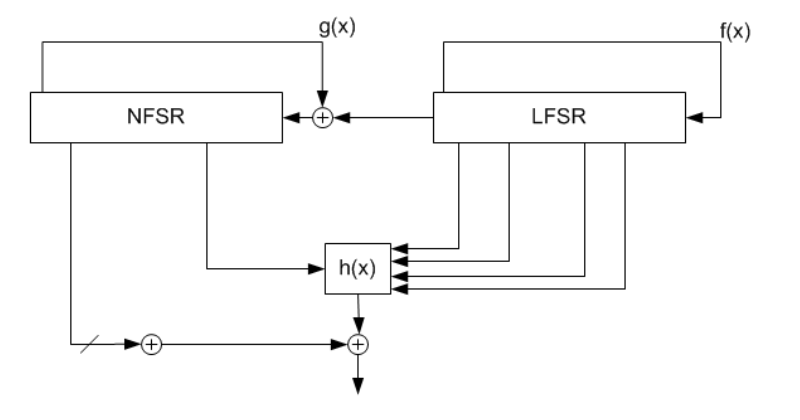
\includegraphics[width=300pt]{p1.png}
\end{center}
\subsection*{Linear Feedback Shift Register (LFSR)}
It is used to generate the initial state of the NFSR and to generate the keystream.\\
LFSR is denoted by $s_{i},s_{i+1},...,s_{i+79}$ \\\\
\textbf{Feedback Polynomial}\\
The feedback polynomial of LFSR is primitive polynomial of degree 80. \\
$f(x) = 1 + x^{18} + x^{29} + x^{42} + x^{57} + x^{67} + x^{80}$ \\\\
\textbf{Update Function}\\
The update function of LFSR is defined as,\\
$s_{i+80} = s_{i+62} + s_{i+51} + s_{i+38} + s_{i+23} + s_{i+13} + s_{i}$ 

\subsection*{Non-Linear Feedback Shift Register (NFSR)} 
It is used to generate the keystream. NFSR is denoted by $b_{i},b_{i+1},...,b_{i+79}$ \\\\
\textbf{Feedback Polynomial}\\
The feedback polynomial of NFSR defined as, \\
$g(x) = 1 + x^{18} + x^{20} + x^{28} + x^{35} + x^{43} + x^{47} + x^{52} + x^{59} + x^{66} + x^{71} + x^{80} + x^{17}x^{20} + x^{43}x^{47} + x^{65}x^{71} + x^{20}x^{28}x^{35} + x^{47}x^{52}x^{59} + x^{17}x^{35}x^{52}x^{71} + x^{20}x^{28}x^{43}x^{47} + x^{17}x^{20}x^{59}x^{65} + x^{17}x^{20}x^{28}x^{35}x^{43} + x^{47}x^{52}x^{59}x^{65}x^{71} + x^{28}x^{35}x^{43}x^{47}x^{52}x^{59}$ \\\\
\textbf{Update Function}\\
The update function of LFSR is defined as,\\
$b_{i+80} = s_i + b_{i+62} + b_{i+60} + b_{i+52} + b_{i+45} + b_{i+37} + b_{i+33} + b_{i+28} + b_{i+21} + b_{i+14} + b_{i+9} + b_i + b_{i+63}b_{i+60} + b_{i+37}b_{i+33} + b_{i+15}b_{i+9} + b_{i+60}b_{i+52}b_{i+45} + b_{i+33}b_{i+28}b_{i+21} + b_{i+63}b_{i+45}b_{i+28}b_{i+9} +
b_{i+60}b_{i+52}b_{i+37}b_{i+33} + b_{i+63}b_{i+60}b_{i+21}b_{i+15} + 
b_{i+63}b_{i+60}b_{i+52}b_{i+45}b_{i+37} + b_{i+33}b_{i+28}b_{i+21}$ 

\subsection*{Output Function}
The input is taken both from the LFSR and from the NFSR. The function is defined as,\\
$h(x) = x_1 + x_4 + x_0x_3 + x_2x_3 + x_3x_4 + x_0x_1x_2 + x_0x_2x_3 + x_0x_2x_4 + x_1x_2x_4 + x_2x_3x_4$ \\
where $x_0$, $x_1$, $x_2$, $x_3$, and $x_4$ correspond $s_{i+3}$, $s_{i+25}$, $s_{i+46}$, $s_{i+64}$ and $b_{i+63}$ respectively. \\
\\
The output function is taken as\\
$z_i = \Sigma_{k \in A}( b_{i+k} + h(s_{i+3}, s_{i+25}, s_{i+46}, s_{i+64}, b_{i+63}))$ \hspace{2cm} $\forall k \in A$\\
where $A = {1, 2, 4, 10, 31, 43, 56}$ 

\subsection*{Key Initialization}
\begin{center}
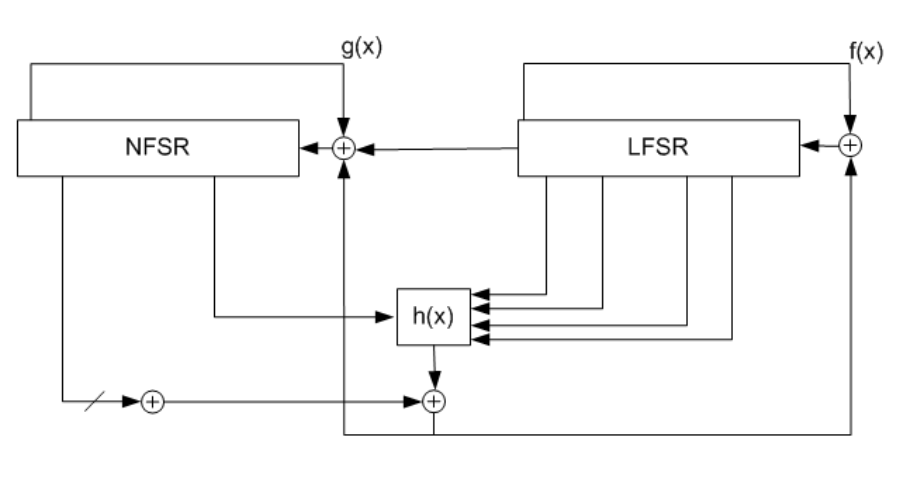
\includegraphics[width=300pt]{p2.png}
\end{center}
\begin{itemize} 
\itemsep 0em
\item The cipher requires initialization with the key and the initialization vector (IV) before generating any keystream.
\item The key bits are denoted by $k$ and IV bits are denoted by $IV$.
\item The key initialization is performed by loading the NFSR with key bits such that $b_i = k_i$, where $0 \leq i \leq 79$.
\item The first 64 bits of the LFSR are loaded with the IV bits such that $s_i = IV_i$, where $0 \leq i \leq 63$.
\item The remaining bits of the LFSR are filled with ones such that $s_i = 1$, where $64 \leq i \leq 79$.
\item The LFSR cannot be initialized to the all-zero state due to the previous step.
\item The cipher is clocked 160 times without producing any running key.
\item Instead of producing the running key, the output function is fed back and xored with the input, both to the LFSR and to the NFSR.
\end{itemize}

\section*{RC4 Stream Cipher}
It is a binary additive stream cipher. It uses a variable sized key ranging from 8 to 2048 bits.\\
\\
RC4 data structure consist of an S-box,\\
$S = (S[0],...,S[N-1])$ \hspace{3cm}where $N = 2^{n}$, each entry is an n-bit integer.\\
$S$ is initialized as the identity permutation, i.e., $S[i] = i$ for $0 \leq i \leq N-1$. \\\\
$K = (K[0],...,K[N-1])$, here each entry is again an $n$-bit integer. \\
The key is repeated in the array $K$ at key length boundaries. \\
K is of size $l$ bytes (typically, $5 \leq l \leq 16$).\\\\
Cipher has two components: \\
1. Key Scheduling Algorithm (KSA) 
\begin{itemize}
\itemsep 0em
\item The KSA (Key Scheduling Algorithm) shuffles the elements of $S$ using the secret key $K$.
\item The PRGA (Pseudo-Random Generation Algorithm) generates pseudo-random keystream bytes using the shuffled permutation.
\item RC4 uses two indices, $i$ and $j$, where $i$ is incremented by 1 (modulo $N$) and $j$ is updated based on $K$ and $S$.
\item The KSA initializes $i$ and $j$ to 0, and $S$ to the identity permutation.
\item $i$ steps across $S$ looping $N$ times, and $j$ is updated by adding the $i$-th entries of $S$ and $K$.
\item Each iteration of KSA ends with a swap of the two bytes in $S$ pointed by the current values of $i$ and $j$.
\end{itemize}
\textbf{Pseudocode :}\\
Input : Secret key array $K[0...N-1]$ \\
Output : Scrambled permutation array $S[0...N-1]$\\
Initialization : \\
for $i=0$ to $N-1$ do \\
\hspace*{0.5cm} $S[i] = i$ \\
\hspace*{0.5cm} $j = 0$ \\
Scrambling : \\
for $i=0$ to $N-1$ do \\
\hspace*{0.5cm} $j = j + S[i] + K[i]$ \\
\hspace*{0.5cm} $Swap(S[i],S[j])$ \\
\\
2. Pseudo-Random Generation Algorithm (PRGA).
\begin{itemize}
\itemsep 0em
\item The Pseudo-Random Generation Algorithm (PRGA) is used in RC4 to generate pseudo-random keystream bytes.
\item The PRGA initializes both $i$ and $j$ to 0.
\item It then loops over four operations in sequence: it increments $i$ as a counter, updates $j$ by adding $S[i]$, swaps the two entries of $S$ pointed by the current values of $i$ and $j$,
\item Finally, it generates a pseudo-random byte of the keystream by xoring $S[i]$ with $S[j]$ and outputs the result.
\end{itemize}
\textbf{Pseudocode :}\\
Input : Key dependent scrambled permutation array $S[0...N-1]$ \\
Output : Pseudocode keystream bytes $z$\\
Initialization : \\
$i = j = 0$ \\
Keystream generation loop : \\
$i = i+1$\\ 
$j = j+1$\\
$Swap(S[i],S[j])$\\
$t = S[i] + S[j]$\\
return $z = S[t]$ 

\section*{Public Key Cryptography}
\subsection*{Diffie-Hellman Key Exchange}
$G \rightarrow $ Cyclic Group \\
$G \rightarrow  <g> $ \\
$|G| = n$ \\\\
\textbf{Alice} \hspace{7.5cm} \textbf{Bob} \\
$0 \leq a \leq n-1 \hspace*{6cm} 0 \leq b \leq n-1$ \\
$K_{a} = g^{a}\xrightarrow{\hspace*{2.75cm}K_{a} = g^{a}\hspace*{2.75cm}} K_{b} = g^{b} $\\
$K_{b} = g^{b}\xleftarrow{\hspace*{2.75cm}K_{b} = g^{b}\hspace*{2.75cm}} K_{a} = g^{a} $ \\
$(K_{b})^{a} = (g^{b})^{a} = g^{ba} \hspace*{4.85cm} (K_{a})^{b} = (g^{a})^{b} = g^{ab}$ \\
Here, Shared secret key is $g^{ab}$.\\
\\
\textbf{Alice} \hspace{7.5cm} \textbf{Bob} \\
Secret key : $a$ \hspace{6.2cm} Secret key : $b$ \\
Public key : $g^a$ \hspace{6cm} Public key : $g^b$ \\
\\
$g^x \rightarrow$ public \\
$x \rightarrow$ secret \\
Based on the property of Group $(G,*) = <g>$, finding $x$ from $g^x$  will be computationally difficult (Discrete log problem).\\
$y = g^x \rightarrow log_{g}y = x $\\
\\

\subsection*{Man in middle Attack}
\textbf{Alice} \hspace{5cm} \textbf{Oscar} \hspace{5cm} \textbf{Bob} \\
$ a \xrightarrow{\hspace*{2.75cm}g^a\hspace{3cm}} c \xrightarrow{\hspace*{2.5cm}g^c\hspace{2.5cm}} b $ \\
$ g^a \xleftarrow{\hspace*{2.75cm}g^c\hspace{3cm}} g^c \xleftarrow{\hspace*{2.5cm}g^b\hspace{2.5cm}} g^b $ \\
\\
The security of sharing $g^a$ and $g^b$ is compromised when a third party is involved in sending data between Alice and Bob.This is because any individual in the middle can generate $g^c$ and share it inside of $g^a$ and $g^b$ with Bob and Alice hence accessing the data.Even without altering the message, a middleman like Oscar can intercept and access the data, making the communication insecure. \\
Also if $g^a$ is very large then computation is hard, To overcome this issue, Square and Multiply algorithm is used.

\subsection*{Square and Multiply Algorithm}
$C = \Sigma_{i=0}^{l-1} C_i 2^i  \hspace*{2cm} C_i \in \{0,1\}$ \\
$C = (C_{l-1},..,C_0)$ \\
Goal is to compute $x^c$. \\
\\
\textbf{Pseudocode}\\
$Z = 1$ \\
for $i=l-1$ to $0$ \\
\hspace*{0.5cm}$Z = Z^2$ \\
\hspace*{0.5cm}if $C_i = 1$ \\
\hspace*{0.8cm} $Z = Z \times x$ \\
return $Z$ \\
\\
\subsection*{RSA}
$\phi(m)$ = number of positive integers $\leq$ $m$ that are co-prime to $m$. \\
For example, $\phi(8) = 4$ because the numbers $1$, $3$, $5$, and $7$ are co-prime to $8$.\\
\\
If $p$ is a prime number then, \\
$\phi(p) = p-1$. \\
$\phi(p^k) = p^k - p^{k-1} = p^k(1-\frac{1}{p})$\\
\\
To have unique characters, it is necessary to have $\gcd(a,m)=1$. \\
If $S = x \bmod m$ and $S = r_1, r_2, \dots, r_m$, then $S_1 = \{ar_1, ar_2, \dots, ar_m \}$. \\
If $ari \equiv arj \pmod m$ and $ri \neq rj \pmod m$, then $\gcd(a,m) = 1$.\\
\\
\textbf{Proof}:\\
Assume $\gcd(a,m) \neq 1$.\\
\\
Then, there exists a prime factor $p$ of $\gcd(a,m)$ such that $p\mid a$ and $p\mid m$. \\
Let $a = ap'$ and $m = mp'$, where $p'$ is the product of the remaining prime factors. \\
Then, $ap'r_i \equiv ap'r_j \pmod{mp'}$.\\
\\
Since $p\mid m$, we can cancel out $p'$ to obtain $ar_i \equiv ar_j \pmod m$. \\
This contradicts the assumption that $ri \neq rj \pmod m$. \\
Therefore, $\gcd(a,m) = 1$.
\end{document}
